\documentclass[sigconf]{acmart}
\usepackage{booktabs}


%% \BibTeX command to typeset BibTeX logo in the docs
\AtBeginDocument{%
  \providecommand\BibTeX{{%
    \normalfont B\kern-0.5em{\scshape i\kern-0.25em b}\kern-0.8em\TeX}}}

%% These commands are for a PROCEEDINGS abstract or paper.
\settopmatter{printacmref=false} % Removes citation information below abstract
\renewcommand\footnotetextcopyrightpermission[1]{} % removes footnote with conference information in 

\acmConference[AEPRO 2024]{AEPRO 2024: Algorithm Engineering Projects}{March 1}{Jena, Germany}

% convert text to title case
% http://individed.com/code/to-title-case/

% that helps you to formulate your sentences
% https://www.deepl.com/translator

\begin{document}

%%
%% The "title" command has an optional parameter,
%% allowing the author to define a "short title" to be used in page headers.
\title[Fast Entity Resolution With Mock Labels and Sorted Integer Sets]{Fast Entity Resolution With Mock Labels and Sorted Integer Sets\\\large Algorithm Engineering 2024 Project Paper}

%%
%% The "author" command and its associated commands are used to define
%% the authors and their affiliations.

\author{Max Mustermann}
\affiliation{%
  \institution{Friedrich Schiller University Jena}
  \country{Germany}}
\email{max.mustermann@uni-jena.de}

\author{Erika Mustermann}
\affiliation{%
  \institution{Friedrich Schiller University Jena}
  \country{Germany}}
\email{erika.mustermann@uni-jena.de}

%% The abstract is a short summary of the work to be presented in the article.
\begin{abstract}

The five-finger pattern \cite{macgilchrist2014}:
\begin{enumerate}
\item \textbf{Topic and background:} What topic does the paper deal with? What is the point of departure for your research? Why are you studying this now?
\item \textbf{Focus:} What is your research question? What are you studying precisely?
\item \textbf{Method:} What did you do?
\item \textbf{Key findings:} What did you discover?
\item \textbf{Conclusions or implications:} What do these findings mean? What broader issues do they speak to?
\end{enumerate}


\end{abstract}

%%
%% Keywords. The author(s) should pick words that accurately describe
%% the work being presented. Separate the keywords with commas.
\keywords{entity resolution, data cleansing, programming contest}


%%
%% This command processes the author and affiliation and title
%% information and builds the first part of the formatted document.
\maketitle

\let\thefootnote\relax\footnotetext{AEPRO 2024, March 1, Jena, Germany. Copyright \copyright 2024 for this paper by its authors. Use permitted under Creative Commons License Attribution 4.0 International (CC BY 4.0).}


\section{Introduction}


\subsection{Background}

\subsection{Related Work}

\subsection{Our Contributions}

\subsection{Outline}



\section{The Algorithm}

\subsection{Internal Representation of Mock Labels}
\label{sub:sec:internal}

In Figure~\ref{fig:integer:sets} we convert the mock labels to sorted integer sets.



\begin{figure}[htbp]
  \centering
  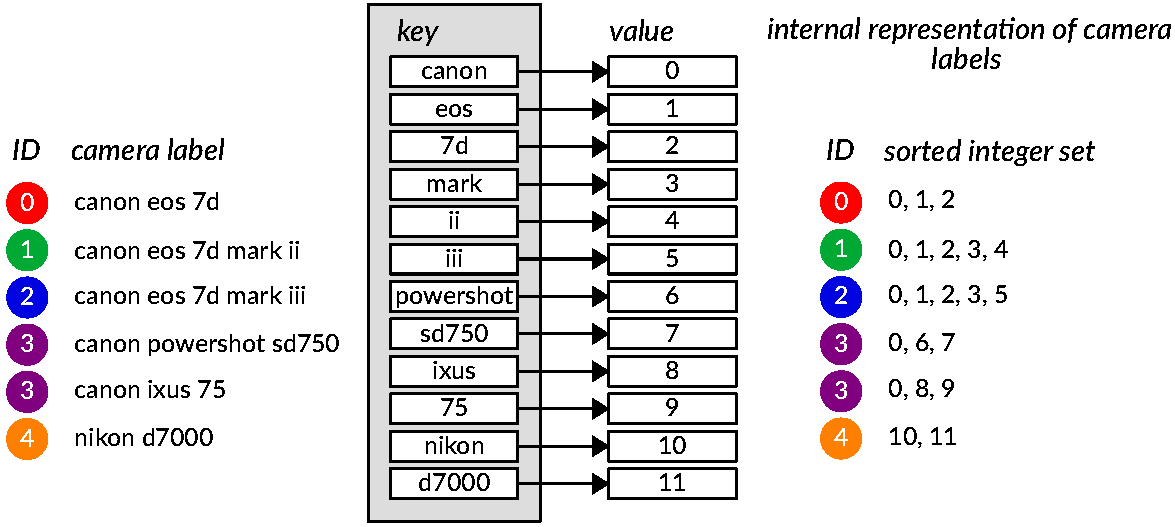
\includegraphics[width=\linewidth]{./graphics/integer_sets.pdf}
  \caption{Conversion of mock camera labels to sorted integer sets. 
We map each unique token (key) in camera labels to a unique value. 
Based on these key-value-mappings, we convert camera labels to sorted integer sets. 
A camera can have different names in different countries. Therefore, repeating IDs reference the same cameras (see, for example, ID=3).} 
  \label{fig:integer:sets}
\end{figure}

\subsection{Efficient Preprocessing of Input Data}
\label{sub:sec:preprocessing}

The following findings are important to speed up preprocessing of the input data:

\begin{itemize}
\item Reading many small files concurrently, with multiple threads (compared to a single thread), takes advantage of the internal parallelism of SSDs and thus leads to higher throughput \cite{Zhuang2016}.

\item C-string manipulation functions are often significantly faster than their C++ pendants. For example, locating substrings with \texttt{strstr} is around five times faster than using the C++ \texttt{std::string} function \texttt{find}.

\item Hardcoding regular expressions with \emph{while, for, switch} or \emph{if-else} statements results in faster execution times than using standard RegEx libraries, where regular expressions are compiled at runtime into state machines.

\item Changing strings in place, instead of treating them as immutable objects, eliminates allocation and copying overhead.

\end{itemize}


\section{Experiments}

Table~\ref{tab:results} shows the running times of the resolution step of the five best placed teams.


\begin{table}[htbp]
  \caption{Comparison of the F-measure and the running times of the resolution step of the five best placed teams. The input data for the resolution step consisted of 29{,}787 in JSON formatted e-commerce websites. Measurements were taken on a
laptop running Ubuntu 19.04 with 16 GB of RAM and two Intel Core i5-4310U CPUs. The underlying SSD was a 500\,GB 860 EVO mSATA. We cleared the page cache, dentries, and inodes before each run to avoid reading the input data from RAM instead of the SSD.}
  \label{tab:results}
\resizebox{\columnwidth}{!}{
  \begin{tabular}{lcrr}
    \toprule
    Team& Language & F-measure & Running time (s)\\
    \midrule
	PictureMe (\textbf{this paper}) &C++& 0.99 & \textbf{0.61}\\
    DBGroup@UniMoRe &Python& 0.99 & 10.65\\
    DBGroup@SUSTech &C++& 0.99 & 22.13\\
    eats\_shoots\_and\_leaves &Python& 0.99 & 28.66\\
    DBTHU &Python& 0.99& 63.21\\
  \bottomrule
\end{tabular}
}
\end{table}


\section{Conclusions}

%%
%% The next two lines define the bibliography style to be used, and
%% the bibliography file.
\bibliographystyle{ACM-Reference-Format}
\bibliography{literature}


\end{document}
\endinput
%%
%% End of file `sample-sigconf.tex'.
